\section{Introduction} 
\label{sec:intro}
Basic-block execution (BBE)

Discussion on single-threaded computing

Energy behavior or O3 and its shortcomings

Performance behavior of O3 and its benefits (speculation and dynamism)

Discussion of related papers that address above issues. items are: 
1) dynamism and speculation computing~\cite{dyn_specul},
2) multi-scalar
3) energy efficient computing (recent papers on this)


\begin{figure}[h]
	\centering
	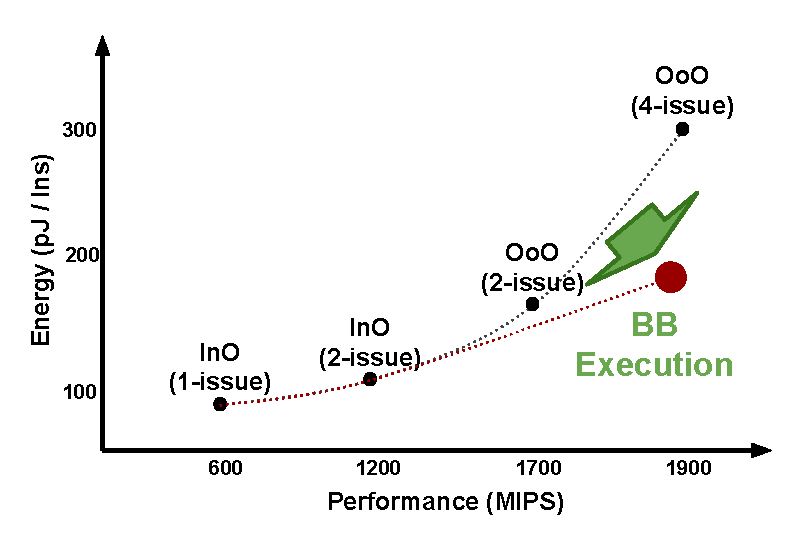
\includegraphics[width=1.0\columnwidth]{fig/energy_perf_insight.pdf} 
	\caption{Energy-Performance trend of recent micro-architectures}
	\label{fig:insight}
\end{figure}


% As described by~\cite{}, the exceptionally high
% performance of out-of-order (OoO) processors is fundamentally due to two key
% attributes: dynamism and speculation.  Lack of either feature can significantly
% impact its performance. 
% 
% The key sources of energy consumption in OoO processors is data-movement and XX
% (back this up).
% 
Dynamic execution and program speculation enable significant single-threaded
performance benefits through effective latency hiding of unpredictable events
such as cache miss and control mis-speculation.  Despite their performance
advantages, these execution models produce significant energy overhead for
keeping track of instruction states and generate substantial on-chip data
traffic; this energy overhead may be acceptable when, in fact, an unpredictable
event stalls the execution flow; otherwise, a statically scheduled program can
perform at least as well as a dynamically generated schedule.

This paper makes the following contributions:
\begin{itemize}
    \item It evaluates the impact of dynamic / static hybrid instruction
    scheduling on energy efficient and high-performance computing. To do so, it
    evaluates coarse-grain execution as a tool to avoid program context tracking
    at instruction granularity.
    \item It evaluates an energy-aware set of compilation strategies including
    local register renaming, block level instruction scheduling, ahead branch
    prediction support.
    \item It provides a new front-end model in which the branch prediction unit
    is only accessed by branch instruction addresses without introducing fetch
    stall bubbles in the pipeline.
    \item It introduces coarse-grain squash with neither context checkpointing
    nor re-order buffer drain support.
    \item It evaluates the performance benefits of the register renaming
    algorithm with one register alias table as a tool for fast program squash
    support and energy efficient renaming.
    \item It provides a 10x shorter re-order buffer model that tracks program
    order at basic-block granularity, enabling bulk instruction commit and fast
    squash restart.
\end{itemize}

Section~\ref{sec:rel_work} covers the related work,
    section~\ref{sec:o3_overhead} discusses the major energy bottlenecks of the
    OoO execution, section~\ref{sec:course_grain} describes our energy
    efficiency vision behind coarse-grain execution, section~\ref{sec:code_gen}
    discusses our energy-aware compilation methodology, section~\ref{sec:uarch}
    provides the Bsaic-block execution model microarchitecture,
    section~\ref{sec:simulation} has the simulation methodology,
    section~\ref{sec:discussion} discusses the results achieved in this work,
    and section~\ref{sec:conclusion} concludes the paper.
